\subsection{Vergleichbarkeit der Ergebnisse}
\label{sec:vergleichbarkeit-der-ergebnisse}

Die im Folgenden präsentierten Modelle unterscheiden sich, wie schon in \autoref{tab:coverage} gezeigt, durch verschiedene Hyperparameter, die zu verschiedenen Werten der Clip-Dauer $\Delta$ führen.
Während des Trainings werden im Trainings- und Validierungsset Samples generiert, deren Länge $\Delta_\text{fit} = \frac{T}{\tau}$ von der Wahl der Hyperparameter $\tau$ und $T$ abhängt.
Um vergleichbare Ergebnisse bei verschiedenen Hyperparametern zu gewährleisten, umfasst das Test-Set hingegen die immer gleichen Samples mit einer festen Clip-Dauer von $\Delta_\text{test}=6$, die sich an der maximalen Länge einer Spielaktion in \gls{sbod} (siehe \autoref{subsec:hyperparameter}) orientiert.

Die Wahl von $\gamma_\tau$ wird während der Evaluation in jedem Fall übernommen, da sie grundlegende Eigenschaften (wie die Geschwindigkeit) der Samples abbildet, auf die das vortrainierte Modell bereits zugeschnitten ist.
Die Test-Samples sind aber immer länger als die Trainings- und Validierungssamples mit $\Delta_\text{fit} < \Delta_\text{test}$.
Um diese Hürde zu überwinden, werden drei verschiedene Methoden verglichen, den Input des zu evaluierende Modells abzuändern:

\begin{description}
    \item[Avg-Consensus]
    Ein Test-Clip wird in mehrere zeitliche Crops segmentiert, die sich gleichmäßig über den gesamten Zeithorizont des Test-Clips verteilen und sich potentiell überschneiden.
    Die Crops werden einzeln inferiert und der endgültigen Score des Clips ergibt sich aus einer Aggregation (consensus function) über alle Crops.
    Als Aggregation wird in diesem Zusammenhang der Durchschnitt pro Klasse ermittelt.
    \item[Max-Consensus]
    Analoge Verarbeitung zu Avg-Consensus, wobei als Aggregation das Maximum pro Klasse berechnet wird.
    \item[Avg-Pooling]
    Der zeitliche Dimension $T$ des Test-Clip wird auf die nötige Anzahl erhöht, um die Test-Dauer zu erreichen.
    Alle trainierten Modelle verfügen über ein dynamischen Avg-\pool-Layer, das die Feature-Maps rechtzeitig wieder auf eine fixe Dimension für die hinteren \fc-Layer projeziert.
    Das Modell aggregiert die Informationen somit intern.
\end{description}

Während des Training werden stets 5-dimensionale Input-Batches $x_\text{fit} \in (B \times \gls{tld:C} \times T \times S \times S)$ verwenden.
Bei der Evaluation wird nun eine weitere Dimension benötigt, um die verschiedenen Crops abzubilden mit $x_\text{test} \in (B \times E \times C \times T \times S \times S)$.
Dabei stell $E$ die Anzahl der zeitlichen Crops dar.

Für ein vortrainiertes Modell mit maximaler Batchgröße $B_\text{fit}$ und Clip-Dauer $\Delta_\text{fit}$, lassen sich unter der Annahmen, dass das Produkt aller Dimension gleich bleibt, die maximalen Dimensionen für $x_\text{test}$ eindeutig ermitteln.
\autoref{eq:eval-dims-consensus} zeigt die Dimension für Avg- und Max-Consensus.

\begin{equation}
    \label{eq:eval-dims-consensus}
    \begin{split}
    E_\text{test}           & = \lceil  \frac{\Delta_\text{test}}{\Delta_\text{fit}}  \rceil \\
    T_\text{test}           & = T_{\text{fit}} \\
    B_\text{test}           & = \lfloor \frac{B_\text{fit}}{E_\text{test}} \rfloor
    \end{split}
\end{equation}

Alternativ werden im Falle des Avg-Pooling die Dimensionen wie in \autoref{eq:eval-dims-pool} gewählt.

\begin{equation}
    \label{eq:eval-dims-pool}
    \begin{split}
    E_\text{test}           & = 1 \\
    T_\text{test}           & = \lceil T_\text{fit} \frac{\Delta_\text{test}}{\Delta_\text{fit}} \rceil \\
    B_\text{test}           & = \lfloor \frac{T_\text{test} }{B_\text{fit} T_\text{fit}} \rfloor
    \end{split}
\end{equation}

\subsection{Vergleich temporärer Aggregationsverfahren}
\label{subsec:initialisierungsphase}

In der ersten Phase der Experimente werden pro Modell vortrainierte (basierend auf Kinetics-400) und öffentlich zugängliche Gewichte in die Architektur geladen.
Das jeweils letzte \fc-Klassifikationslayer wird durch ein neues mit 32 Output-Klassen ausgetauscht und einzeln für einen Zyklus (siehe \autoref{subsec:trainingsschleife}) mit etwa $\Theta_\text{train} = 100$ Samples pro Klasse nachtrainiert.
\Dh alle übrigen Layer des Modells bleiben unverändert.
Erst in einer späteren Iteration werden alle Layer in einem zweiten Zyklus nachtrainiert.
Diese Instanzen werden nachfolgend als Baseline-Modelle bezeichnet.

Für alle der drei Baseline-Modelle wird nach Abschluss des zweiten Zyklus evaluiert welches der oben genannten Aggregationsverfahren für die Test-Samples am besten geeignet ist.
Pro Backbone wird das Test-Set pro Verfahren getestet.
\autoref{fig:consensus} zeigt verschieden Metriken für jede der Aggregationen.
Die Metriken werden im Verhältnis zu den Ergebnissen des Validierungssets aufgetragen.
\Dh eine Metrik von 1 entspricht dem gleichen absoluten Wert der Metriken im Validierungsset, eine Metrik von 0.5 entspricht einem halb so hohen Wert.

\begin{figure}[htbp!]
    \centering
    \begin{subfigure}{.33\textwidth}
        \centering
        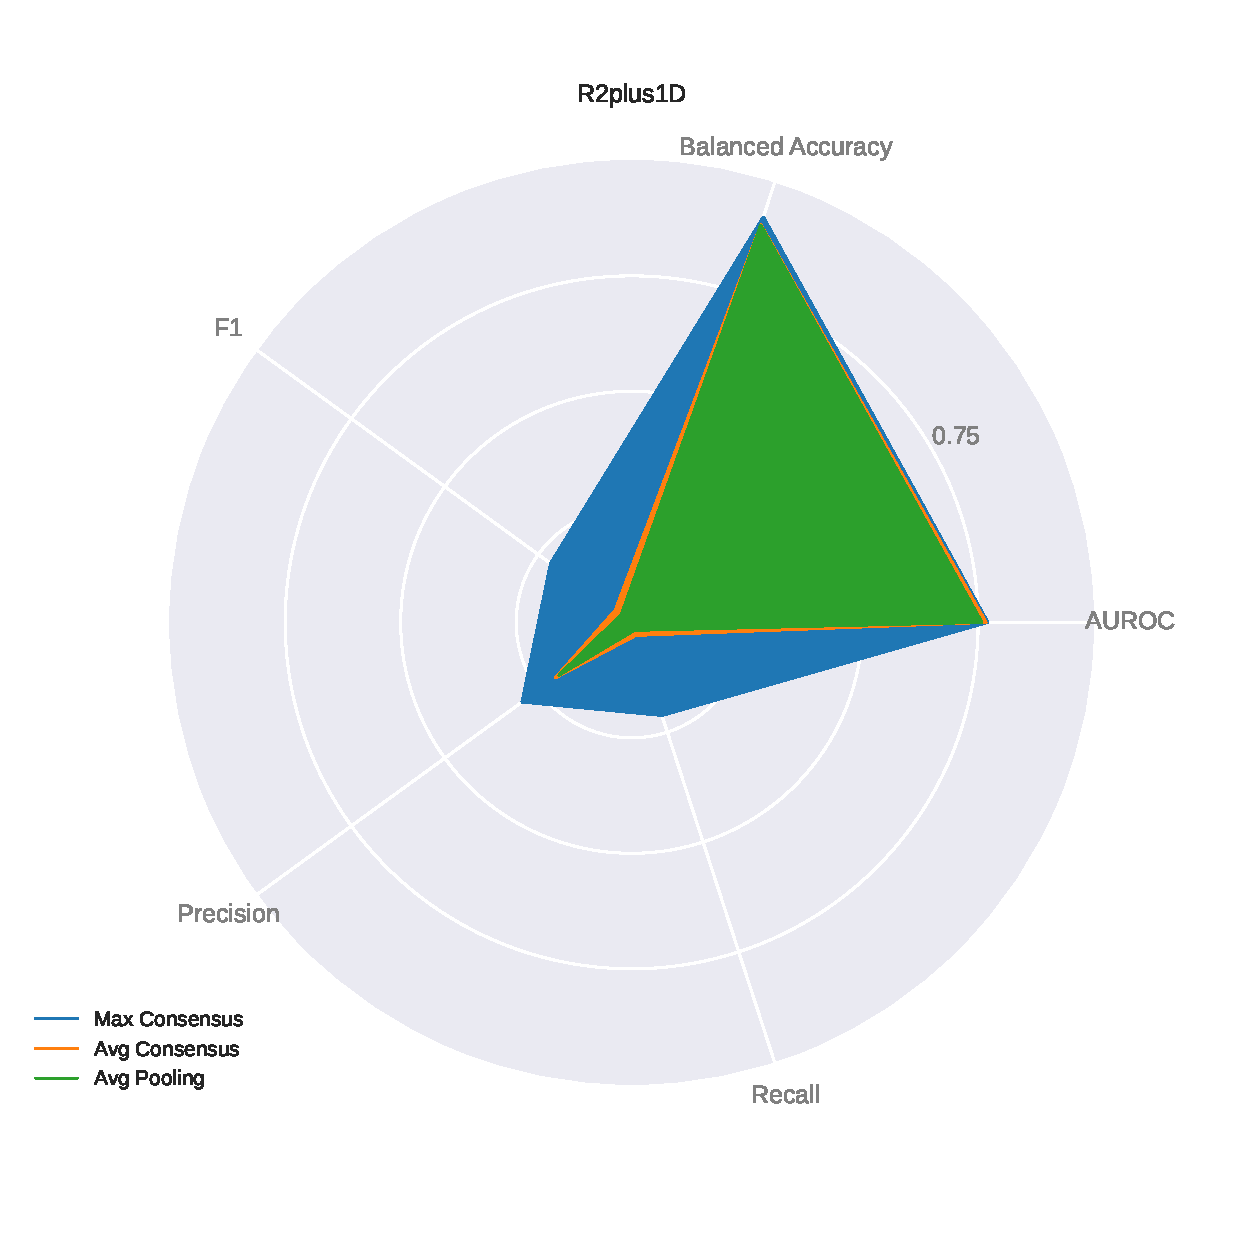
\includegraphics[width=0.9\textwidth, keepaspectratio, interpolate]{img/07_consensus_R2plus1D.eps}
    \end{subfigure}%
    \begin{subfigure}{.33\textwidth}
        \centering
        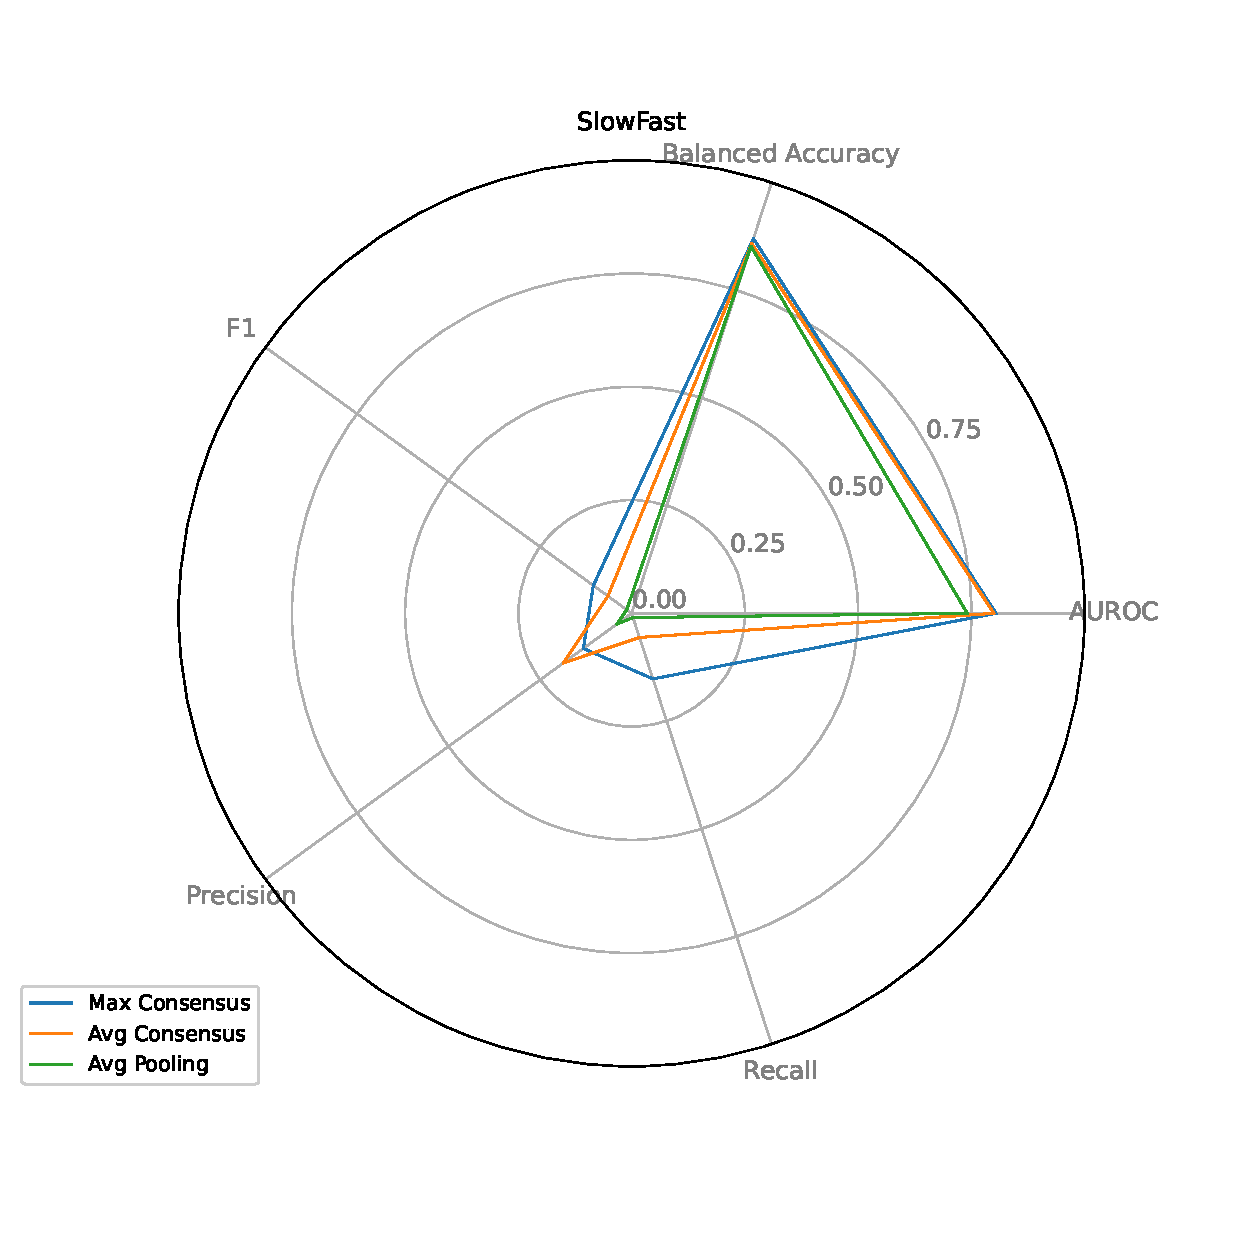
\includegraphics[width=0.9\textwidth, keepaspectratio, interpolate]{img/07_consensus_SlowFast.eps}
    \end{subfigure}%
    \begin{subfigure}{.33\textwidth}
        \centering
        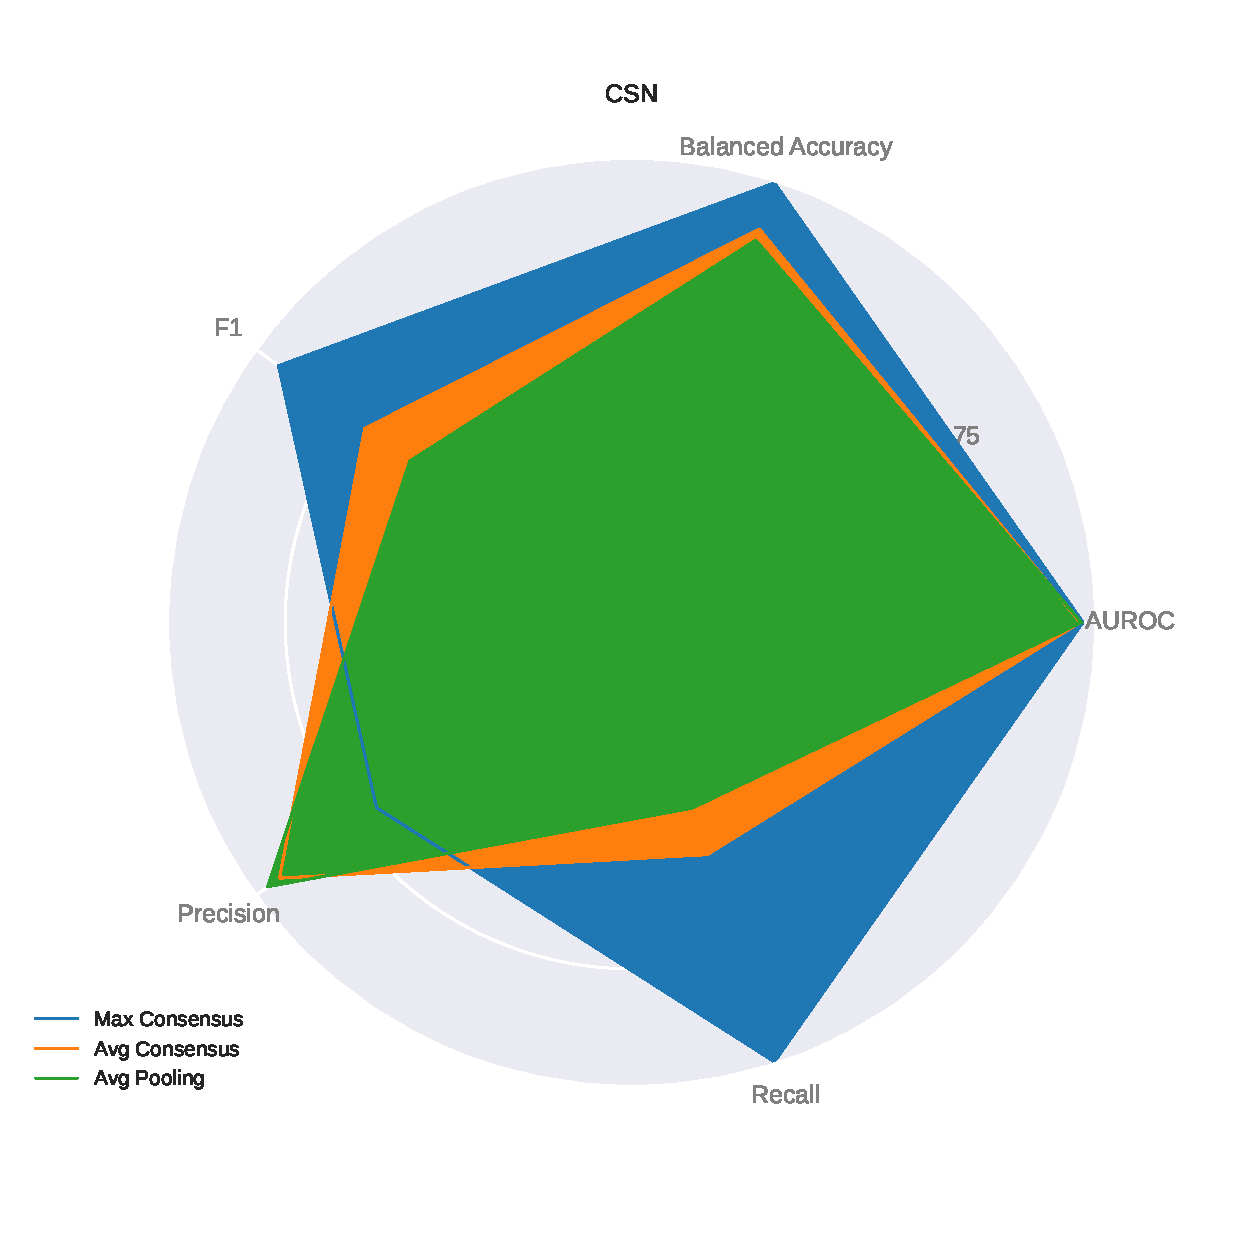
\includegraphics[width=0.9\textwidth, keepaspectratio, interpolate]{img/07_consensus_CSN.eps}
    \end{subfigure}
    \caption{Vergleich von Aggregationsmethoden}
    \label{fig:consensus}
\end{figure}

Die Avg-Aggregation weist in den meisten Fällen eine knapp höhere Precision und Accuracy auf, während die Max-Aggregation einen deutlich höheren Recall, eine leicht höhere AUROC und Balanced Accuracy und in den meisten Fällen einen leicht höheren F1-Score.
Die Ergebnisse lassen sich zum Teil dadurch erklären, dass die Scores durch die Mittelung der Avg-Aggregation immer niedriger sind als die Scores in der Max-Aggregation, wodurch die Anzahl aller Positives insgesamt abnimmt.
Die Avg-Aggregation ist also deutlich sensibler gegenüber False Positives.

Dennoch wird die Max-Consensus-Aggregation als primäre Aggregation für den weiteren Verlauf festgelegt.
Zum einen, da die Metriken im Schnitt einen besseren Kompromiss darstellen.
Zum anderen, da sie die Realität logisch abbildet:
Enthält ein Clip von 10 Sekunden zwei Aktionen -- die eine Aktion ganz zu Beginn und die andere Aktion kurz vorm Ende, ist die erste Aktion nicht im letzten Chunk und die zweite Aktion nicht im ersten Chunk sichtbar.
Die Max-Aggregation kann derartige Zustände erkennen, da die Maxima sich auf die lokalen Stellen im Clip beziehen, während die Lokalität bei der Avg-Aggregation verwässert und ein hohes Maximum leicht durch weitere niedrige Scores überstimmt werden kann.
